\chapter{Building Blocks}
\label{chap:2}

In this section, we will discuss the primary building blocks to help us construct the $\plonk$ protocol. First, let us start with a very rough overview. Say there exists a problem $\prover$. The prover knows a solution $\witness$ to $\prover$ and wants to convince the verifier that he knows the solution. How will he do it without revealing the solution? Let there be a program that checks solutions to $\prover$ and outputs 0 if the provided solution is valid. This program could be compiled into an arithmetic circuit $\CRKT$. Now, the prover aims to convince the verifier that, for some public input $\publicinput$, there exists solution $\witness$ (witness) such that $\CRKT(\witness, \publicinput) = 0$. In other words, the prover wants to convince others that the program for checking $\prover$ would accept his solution. This only works under the assumption that the verifier believes that the circuit $\CRKT$ correctly checks solutions to $\prover$, so the $\CRKT$ is public for anyone to inspect.

\begin{example}
    Say the prover knows a solution for an instance of a Sudoku problem, and there is a program that checks if the Sudoku is filled validly. The public input $\publicinput$ to this problem are the board's dimensions and pre-filled numbers. The prover knows how to fill the rest of the board, and this information is stored in the witness $\witness$, which is private. To convince the verifier that $\CRKT(\witness, \publicinput) = 0$, the proof should say that the circuit was executed validly. The proof will be encoded in polynomials, and we will ensure it reveals nothing about the $\witness$.
\end{example}

\hl{explain image}

\begin{figure}[H]
    \centering
    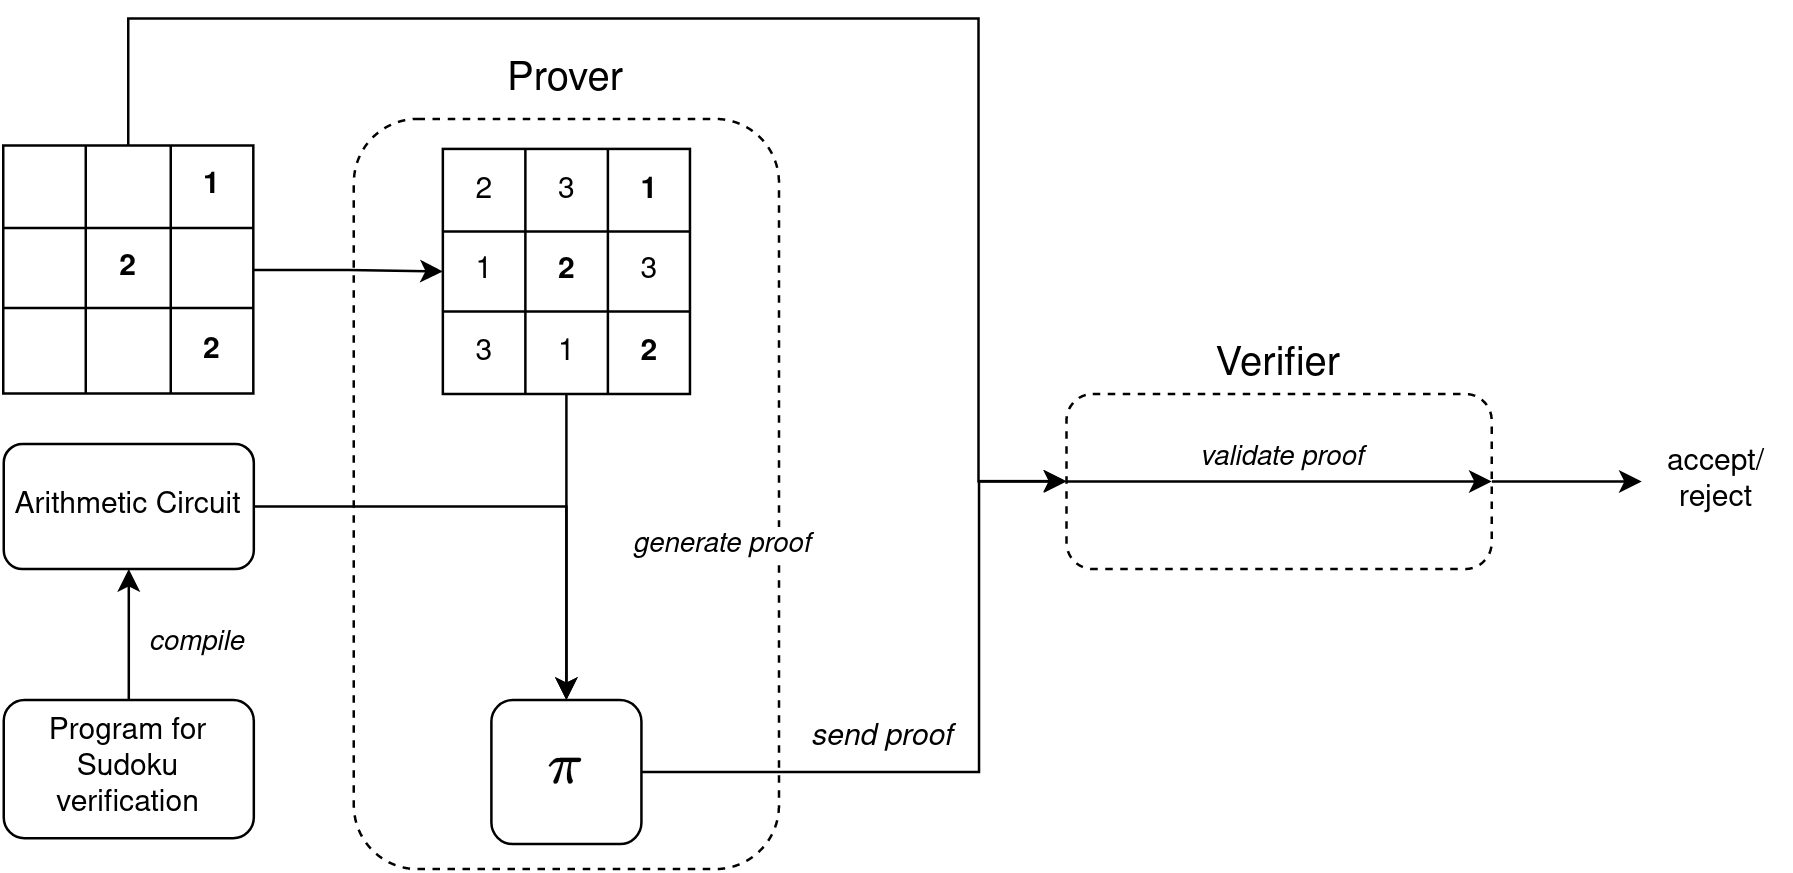
\includegraphics[width=1\linewidth]{figures/sudoku.drawio.png}
    \caption{Sudoku Example}
\end{figure}

% \begin{enumerate}
%     \item Encode circuit with secret and public parameters into polynomials
%     \item Generate a proof that this encoding was indeed done correctly
%     \item Verify that the proofs are valid
% \end{enumerate}



% %%%  ===========================================================================
% %%%  ===POLYNOMIALS=============================================================
% \section{Polynomials}
% % % \hl{reference how snarks work}
% Polynomials are mathematical objects studied for centuries, throughout this time we have figured out many nice and even some useful properties about them. One might ask what is so special about polynomials and it turns out a lot. They serve as a good tool for representing end encapsulating circuits. Let's show a simple observation:

% \begin{lemma}{Intersection of polynomials} \newline
%     Arbitrary two polynomials in form $a_0 + a_1x + a_2x^2 ... a_nx^n = 0; b_0 + b_1x + b_2x^2 ... b_m x^m = 0$ where both $n, m \leq d \in \mathbb{N}$ intersect in no more than $d$ points.
% \end{lemma}

% \begin{proof} \newline
%     To find the intersection points we need to solve equation $a_0 + a_1x + a_2x^2 ... a_nx^n = b_0 + b_1x + b_2x^2 ... b_m x^m$ which will produce yet another polynomial of degree $max(n,m) \leq d$. From the Fundamental Theorem of Algebra we know that a polynomial of degree $d$ cannot have more than $d$ roots.
% \end{proof}

% This a simple yet incredibly crucial observation for most of the proofs that will be carried out in this article. You can think about it as a tool for probabilistic polynomial identity testing, thanks to which we can effectively compare of two polynomials just by evaluating them at a uniformly random point. If polynomials are different we know they could intersect in at most $d$ points. The probability of randomly picking one of these points is $d$ divided by size of the domain. Depending on reasonably chosen parameters usually give negligible chances to guess the point correctly. Keep in mind the the domain size is given by $\lambda$. The observation can be generalized on multi-variate polynomials by Schwartz-Zippel lemma. % % \hl{include citation} To better understand how it works we will look at series of toy protocols, where we improve their faults in iterative manner. We will start with the most simple and crappy one:

% \begin{example} \textit{Polynomial Identity Check}

%     There is a verifier who knows some polynomial $p(x)$ and prover who wants to claim that he also knows coefficients of the polynomial $p(x)$. Say the polynomial has degree $d$ and the domain or evaluation range is $[1, 2^n]$. The prover could convince verifier as follows:
    
%     \begin{enumerate}
%         \item $V$ samples random point $r \in [1, 2^n]$
%         \item $V$ sends the point $r$ to $P$
%         \item $P$ sends back evaluation $p(r)$
%         \item $V$ locally computes $p(r)$ compares to what he got from $P$
%     \end{enumerate}    
% \end{example}

% With each $i$ iterations of this protocol the prover has probability of $(\frac{d}{2^{\lambda}})^i$ of guessing correctly. While this protocol is an interesting proof of concept, by itself it does not achieve much. Both of the parties know the same polynomial the only advantage is that the verifier does not compare coefficients of the polynomial but just one point. What might sound a bit more interesting is that a prover might be able to show that his polynomial $p(x)$ can be factored by $t(x)$ into $p(x) = t(x)h(x)$. 

% \begin{example} \textit{Polynomial Factor Check}

%     P wants to convince $V$ that he knows a polynomial $p(x)$ of degree $d$ with factor $t(x)$. In this protocol $P$ does not want to share $p(x)$ but wants to prove $p(x) = t(x)h(x)$, so naturally $V$ knows $t(x)$.
%     \begin{enumerate}
%         \item $V$ samples a random point $r$
%         \item $V$ sends the point $r$ to $P$
%         \item $P$ performs polynomial division $h(x) = \frac{p(x)}{t(x)}$ and sends evaluations of $p(r), h(r)$ to back to $V$
%         \item $V$ locally evaluates $t(r)$ and checks if $p(r) = t(r)h(r)$
%     \end{enumerate}
% \end{example}

% The protocol relies on the fact that $P$ is able to divide $p(x)$ if and only if $t(x)$ indeed is co-factor. Now we have a protocol in which the verifier is not revealed polynomial $p(x)$ and can relatively succinctly verify if it has some factor so all look good. Or does it? Well, no this protocol is terrible. The verifier gets to know some information about $p$ and that is the evaluation at $r$ and what is much worse the $P$ can cheat very easily in number of different ways:

% \begin{enumerate}
%     \item $P$ does not need to know the coefficients of $p$. He can quite easily calculate evaluation $t = t(r)$ and choose $h(r)$ such that $p(r) = t(r)h(r)$, without the verifier knowing.
%     \item $P$ nothing stops the prover from changing the $p$ on the fly. He know $r$ therefore, it is easy to construct any polynomial which has one shared polynomial with $t(r)h(r)$.
%     \item Nothing is constraining the $P$ to use polynomial of degree $d$. Prover can cheat by using polynomial $\widetilde{p}(x) = p(x)h'(x)$ with arbitrary $h'(x)$ that has bigger degree and also satisfies the factor check.
% \end{enumerate}

% The first two exploits possible because the prover knows $r$ and $t(r)$, thus he can temper with the protocol. Instead we would like to provide encrypted $r$ to the prover, so that he can use it as black box but does not know the real value. We will tackle this problem later by introducing homomorphic encryption, first we need a some understanding of elliptic curves.

\section{Elliptic curves}
The discussed elliptic curves will be over a finite field $\field$ where each for each point $(x, y) \in \field^2$. An elliptic curve is defined as $f(x,y): y^2 = x^3 + ax + b$ with parameters $a, b \in \field$. Points of the curve define a group $\mathbb{G}$ with a neutral element point at infinity $(0, 0)$ and $(x, -y)$ as the inverse element to $(x, y)$. In the following chapters, we will use multiplicative notation, and exponentiation will denote repeated application of the group operation.  We also denote $G$ a generator of the group $\mathbb{G}$. 

\hl{define DLP}

This group is especially interesting due to the hardness of the discrete logarithm problem (DLP), which is considered hard over sufficiently large $\field$. For this reason, $|\field|$ will be viewed as a security parameter of the $\plonk$ protocol. We will rely on the hardness of DLP on elliptic curves, which is standard in many modern cryptographic protocols.


\subsection{Elliptic Curve Arithmetic}
\label{sec:ec-arithmetic}

Given $G^a, G^b$, anyone can perform the operations listed below. However, it is very hard to extract $a, b$ due to DLP. That allows the prover to send some encoded values to the verifier, who will be able to perform arithmetic checks without discovering the original values.

\begin{table}[H]
    \centering
    \begin{tabular}{|l|l|l|l|}
    \hline
    \textbf{Operation}             & \multicolumn{1}{c|}{\textbf{Inputs}} & \textbf{Computation}            & \textbf{Result}    \\ \hline
    Addition              & $G^a, G^b$                  & $G^a \cdot G^b$        & $G^{a+b}$ \\ \hline
    Subtraction          & $G^a, G^b$                  & $G^a \cdot (G^b)^{-1}$ & $G^{a-b}$ \\ \hline
    Scalar multiplication & $G^a, \text{scalar } s$      & $(G^a)^s$              & $G^{as}$    \\ \hline
    Polynomial evaluation &
      \begin{tabular}[c]{@{}l@{}}$\{G, G^{a}, \ldots G^{a^n}\}$ \\ $f(x) = c_0 + c_1x + \ldots c_n x^n$\end{tabular} &
      $\prod_i (G^{a^i})^{c_i}$ &
      $G^{f(a)}$ \\ \hline
    \end{tabular}
\end{table}

The first two operations, addition and subtraction, follow from the definition of the group, and scalar multiplication is just a generalization of the exponentiation. For polynomial evaluation, take arbitrary polynomial $f(x) = c_0 + c_1 x + c_2 x^2 + c_3 x^3 + ... + x^n$ of degree bound $n$. The evaluation of $f(x)$ at some point $a$ can be written as 
$$G^{f(a)} = G^{c_0 + c_1 a + c_2 a^2  + ... + c_k  a^n} = (G^{a^0})^{c_0} \cdot (G^{a^1})^{c_1} \cdot (G^{a^2})^{c_2} \cdot \ldots (G^{a^k})^{c_n} = \prod_{i=0}^n (G^{a^i})^{c_i}$$



% \subsection{Homomorphic Encryption (inspiration how snarks work)}
% Remember the problem from example 2? Now we have all the tools to improve this protocol. We will use encryption function $E(r) = g^r$ where $g$ is a generator of elliptic curve group. Encrypting polynomial evaluated in $r$ with coefficients $c_i$ could be done as $E(r^i)^{c_i} = g^{r^i c_i}$. Evaluation of a polynomial will be denoted as: $E(p(r)) = g^{p(r)} =  (g^1)^{c_0} \cdot (g^{r^1})^{c_1} \cdot (g^{r^2})^{c_2} \cdot \ldots \cdot (g^{r^d})^{c_d}$. In order to make this more clear let's look at a specific example. Say we would like the prover to evaluate polynomial $p(x) = x^3 - 3x^2 +3x$ on the point $r$ without directly revealing $r$. Fist we need to encrypt values $E(r^3), E(r^2), E(r)$ which will be sent to prover. He can then reconstruct the polynomial as follows:

% $$E(r^3)^1 \cdot E(r^2)^{-3} \cdot E(r^3)^2$$
% $$g^{(r^3)^1} \cdot g^{(r^2)^{-3}} \cdot g^{(r^3)^2}$$
% $$g^{r^3 - 3r^2 + 2r}$$


% Given values $E(r^3), E(r^2), E(r)$ can now calculate evaluations $g^{p(r)}, g^{h(r)}$ in the encrypted space. The verifier will also validate the result in encrypted space by checking is $g^{p(r)} = g^{h(r)}g^{t(r)}$. These conditions make life of a dishonest prover much harder, because now he does not know much about the secretly sampled value $r$. % % \hl{more rigorou explanation for why it is harder}
% We have now greatly limited the possibilities of cheating the protocol is still not sound. 

% Remember that there was also a third point, which said that there is nothing constraining the prover to using polynomial of a different degree. Although we have restricted the prover in selection of powers of $r$ we have not restricted him to using them. That is why the verifier need a prove that only the supplied encryption were used to calculate $g^{p(r)}, g^{t(r)}$ and nothing else.


\subsection{Elliptic curve pairing}
\hl{add explanation of groups}

Pairing $e$ is in essence deterministic mapping to another group $e: \mathbb{G}_1 \times \mathbb{G}_2 \rightarrow \mathbb{G}_t$. To be more specific, it is a bilinear mapping that takes two encrypted elements from the source group and combines them into an element of the target group. Since this is a complex topic, we will treat the pairing as a black box; for a more detailed explanation, we refer the reader to \cite{ec-pairings}. For the purposes of this work, it will be sufficient to know that curve pairings have the following properties $\forall a, b \in \field$:
$$e(G_1^a, G_2^b) = e(G_1^b, G_2^a) = e(G_1^{ab}, G_2^1) = e(G_1^1, G_2^{ab}) = e(G_1^1, G_2^a)^b = e(G_1^1, G_2^1)^{ab}$$

In \Cref{sec:ec-arithmetic}, there is no way to calculate $G^{a \times b}$ from $G^a, G^b$. We will use curve pairings to "emulate" this operation $e(G_1^a, G_2^b) = G_t^{ab}$. Note that the operation cannot be performed more than once because the result is in a different target group. Thus, we will be allowed to use this operation in the $\plonk$ protocol only a single time. Not all elliptic curves are pairing-friendly, and this property is rather rare.

\subsection{Multi-scalar Multiplication}
Polynomial evaluation can be performed via multiscalar multiplication (MSM), where elements $\{G, G^a, G^{a^2}, \ldots, G^{a^n}\}$ are pairwise multiplied by scalars $\{c_0, c_1, c_2, \ldots, c_n\}$ and eventually summed. In the group $\mathbb{G}$, the scalar multiplication $(G^{a^i})^{c_i}$ is defined as $c_i$ times repeated group operation $G^{a^i} \cdot G^{a^i} \ldots G^{a^i}$. When dealing with fields in order hundreds of bits, this becomes expensive, and this operation is a major bottleneck of $\plonk$ and many SNARK protocols.

To make this operation faster, it is possible to calculate the elements using the \textit{square and multiply} version, which can be described as:

\begin{equation*}
    (G^{a_i})^n = 
    \begin{cases}
        ((G^{a_i})^2)^{n/2} & 2 \mid n \\
        G^{a_i}((G^{a_i})^2)^{(n-1)/2} & 2 \nmid n 
    \end{cases}
\end{equation*}

The naive way needs to perform $n$ group operations to calculate $(G^a_i)^n$ while \textit{square and multiply} achieves the same result in $\bigO{\log_2{n}}$. The resulting complexity of MSM is $\bigO{n \times  \log_2{\max_i{c_i}} }$.
% $n-1 + \lceil \log_2{c_0} \rceil, \lceil \log_2{c_1} \rceil, \ldots \lceil \log_2{c_n} \rceil \rightarrow \bigO{n \times \lceil \log_2{\max_i{c_i}} \rceil}$. 

\hl{make sure the assumption that the field is much bigger than the degree of the polynomials}
\hl{make simpler delete lambda}
A more efficient way is to use Pipenger's algorithm \cite{Pippengers} with complexity $\bigO{\lambda\frac{n}{\log_2(n)}}$ where $\lambda$ is dependent on the algorithm parameters. There are possible improvements to this algorithm in the form of precomputation and parallelism. In practice, there is also an effort to create a hardware-accelerated version of MSM, described in PipeMSM \cite{pipeMSM}.
% ==============================================================================
% ===POLYNOMIALS================================================================
% ==============================================================================
\section{Polynomial toolkit}

\subsection{Comparing polynomials}
\label{comparing-poly}

Effective comparison of polynomials is one of the building blocks of $\plonk$. We can test if two polynomials are equal just by comparing them at a uniformly random point. 
\begin{theorem}
\label{theorem:poly-intersection}
    Arbitrary two non-identical polynomials $a_0 + a_1x + a_2x^2 ... a_nx^n; b_0 + b_1x + b_2x^2 ... b_m x^m$, where both $n, m \leq d \in \mathbb{N}$ intersect in no more than $d$ points.
\end{theorem}{Intersection of polynomials}

\begin{proof}
    An intersection point $\gamma$ such that $$a_0 + a_1 \gamma + a_2 \gamma^2 \ldots a_n \gamma^n = b_0 + b_1 \gamma + b_2 \gamma^2 \ldots b_m \gamma^m,$$ 
    is a root of the following polynomial of degree $max(n,m) \leq d$
    $$a_0-b_0 + (a_1-b_1)x + (a_2-b_2)x^2 \ldots (a_n - b_n)x^n = 0.$$
    From the Fundamental Theorem of Algebra, we know that a polynomial of degree $d$ cannot have more than $d$ roots.
\end{proof}

If two polynomials are identical, then $\forall x: p(x) = q(x)$, so determining identity based on evaluation at a random point is correct. Two polynomials with different coefficients can be equal at intersection points, so this approach has a soundness error rate. Based on \Cref{theorem:poly-intersection}, two non-identical polynomials might intersect in almost $d$ points, so the probability of randomly selecting one of the intersection points is $\frac{d}{\text{domain size}} = \frac{d}{|\field|}$. This probability is considered negligible. For example, the commonly used elliptic curve $BLS12-381$ has order $\approx 2^{381}$. The failure rate is small enough for most practical purposes, so we can compare two polynomials just by a single evaluation.

\hl{what is usually d give an example}

A multivariate version of the previous observation could be proved by the Schwartz-Zippel lemma \cite{schwartz-lemma}.

\begin{lemma}
\label{sz lemma}
    For domain $D \in \field$ and a polynomial $f(x_1, x_2, \ldots x_n) \in \field[x_1, \ldots, x_n]$ with degree bound $d$ and  independently uniformly at random selected $(r_1, r_2 \ldots r_n) \in D^n$ it holds:
    $$\prob{f(r_1, r_2 \ldots r_n) = 0} \leq \frac{d}{|D|}.$$
\end{lemma}


\subsection{Evaluation domain}
To create the evaluation domain, we use the primitive $n$-th root of unity $\omega \in \field$ for which it holds that $\omega^n = 1$ and $\forall 1 \leq i < n: \omega^i \neq 1$. The evaluation domain $H$ will be constructed as $$H = \{1, \omega, \omega^2 \ldots \omega^{n-1}\}.$$

This domain will be especially useful because it allows for a sparse representation of certain polynomials. This results in numerous benefits, such as faster polynomial evaluation.

\begin{definition}[Vanishing polynomial]
    Denote $Z_H(x)$ the vanishing polynomial for the domain $H$ such that $\forall x \in H: Z_H(x) = 0$ and deg $deg(Z_H) = |H|$.
\end{definition}

Since the vanishing polynomial has roots as the elements of $H$, it could be written as: $$Z_H(x) = (x-1)(x-\omega)(x-\omega^2) \ldots (x-\omega^{n-1}).$$
However, the domain $H$ also allows for a sparse representation of this polynomial $Z_H(x) = x^n-1$. To observe that this holds, we verify $$\forall x \in H: x^n-1 = (\omega^i)^n - 1 = (\omega^n)^i - 1 = 1^i - 1 = 0.$$



    
\subsection{Lagrange basis}
In the $\plonk$ paper, interpolation is performed using the Lagrange basis.

\begin{definition}[Lagrange basis]
    We denote by $L_i$ the $i$th polynomial of the Lagrange basis over $H$ as:
    $$
    L_i(x) = 
        \begin{cases} 
            1 & x = \omega^i \\
            0 & \text{otherwise}
       \end{cases}
    $$
\end{definition}

Given a vector $v = [v_0, v_1, \ldots ,v_{n-1}]$, we interpolate it over the domain $H$ via the polynomial:$$v(x) = \sum_{i=0}^{n-1}v_iL_i(x).$$

The Lagrange basis can be expressed as:  $$L_i(x) = \prod_{k \in H, k \neq \omega^i} \frac{x-k}{\omega^i-k}.$$

The properties of this polynomial are easy to observe. When $x \in H \setminus \{ \omega^i \}$ is plugged into $L_i(x)$, then there is exactly one fraction for which $k = x$, which makes the product 0. If $x = \omega^i$, the consequence is even more trivial because all of the fractions would result in $\frac{\omega^i-k}{\omega^i-k} = 1$, and since $k \neq \omega^i$, $L_i(\omega^i)$ results in 1.

Due to the choice of the evaluation domain, the Lagrange basis also has a sparse representation as presented in \cite{BarycentricLagrange}. 
$$L_i(x) = \frac{b_iZ_H(x)}{x - \omega^i},$$
$$b_i = \prod_{k \in H, k \neq \omega^i} \frac{1}{x_i - x_k}.$$

Notice that each $b_i$ depends only on the elements of the domain $H$. So, all of the values $b_i$ could be precomputed.

%%%  ===========================================================================
%%%  ===COMMITMENT SCHEME=======================================================
\section{Polynomial Commitment Scheme}
A commitment scheme is a cryptographic primitive that makes it possible to commit to a piece of information, ensuring that it remains unchanged throughout the process of verification. One motivation for this mechanism is to prevent the prover from generating proofs depending on the verifier's queries. In the context of $\plonk$, we will rely on the polynomial commitment scheme, where the prover knows the coefficients of some polynomial $f(x)$ and wants to prove evaluation of $f$ at a point given by the verifier. 

A standard polynomial commitment scheme has the following procedures:
\begin{enumerate}
    \item $\mathsf{Setup(\secparam)} \rightarrow \publicparameter$: generate public parameters.
    \item $\mathsf{Commit}(f, \publicparameter) \rightarrow c$: calculate commitment $c$ which binds $\prover$ to the polynomial $f(x)$.
    \item $\mathsf{Open}(z, \publicparameter) \rightarrow (v, \pi):$ given the challenge $z$, $\prover$ returns a pair $(v, \pi)$, where $\pi$ is the proof that $v = f(z)$.
    \item $\mathsf{Verify}(\publicparameter, c, z, v, \pi) \rightarrow \mathsf{accept/reject}$: $\verifier$ checks validity of the claim $f(z) = v$.
\end{enumerate}

\procedureblock{Polynomial Commitment Scheme}{    
    \textbf{Prover } \prover \>\> \textbf{Verifier } \verifier \pclb
    \pcintertext[dotted]{Scheme Setup}
    \mathsf{Commit} \> \sendmessageright*[6cm]{c} \> \\
    \> \sendmessageleft*[6cm]{z} \> z \gets \field \\
    \mathsf{Open} \> \sendmessageright*[6cm]{(v, \pi)} \> \\
    \> \> \mathsf{Verify} \\
    % \>\> \pcreturn accept/reject
}

\hl{odkaz an diagram}
We will require that the commitment is \textit{binding} and \textit{hiding}. Loosely speaking, binding means that the commitment binds the prover to a specific polynomial. Hiding property suggests that the prover does not discover the coefficients of the polynomial $f(x)$. We will define it more formally.

\begin{definition}{Evaluation binding}
    guarantees that any efficient prover is unable to generate a convincing $\pi$ for $v = f(z)$ and $\pi'$ for $v' = f(z)$.
\end{definition}

Computational hiding property says that for polynomial $f(x)$ and its commitment $c$ and any efficient $\adv$, the polynomial $f(x)$ is computationally indistinguishable from a randomly chosen polynomial. We will achieve the hiding of the scheme in \Cref{sec:blinding} with a stronger property — zero-knowledge.


The next notion we formalize ensures that if the verifier accepts the proof, the prover needs to have knowledge of the committed polynomial.

\begin{definition}{Extractable scheme}
    guarantees that for all efficient provers $\prover$ that takes as input public parameters, degree bound $d$ and outputs commitment $c$ $\exists$ efficient extractor algorithm $\extractor$ that has the same input as $\prover$ and produces polynomial $f(x)$ of bound $d$ explaining all of $\prover$ answers to evaluation queries.
    % such that evaluation queries on $f(x)$ correspond to answers of $\adv$ to these queries.
\end{definition}

The extractability of a polynomial commitment is stronger than binding as it was with soundness and knowledge soundness in \Cref{prelim}. It guarantees that for any efficient prover capable of passing all of the checks, the prover must actually “know” a
polynomial p of the claimed degree that explains its answers to all evaluation queries.

% Extractability suggests that the prover needs to have knowledge of $f(x)$ and it can be extracted from him. That follows from the fact that $E$ is efficient and therefore an efficient $\mathcal{A}$ can afford to run it. Since $E$ does not know anything more than $\mathcal{A}$ and can produce $f(x)$ that can use $E$ to get knowledge of $q$, which passes all queries.


\subsection{KZG Polynomial commitment scheme}
The KZG polynomial commitment scheme, based on the pairing (elliptic curve) group, was introduced in \cite{KZG}. It has constant proof size and requires a trusted setup. There are other ways to design polynomial commitment schemes, such as \cite{fri} based on hash functions. We will explain KZG since it is used in the $\plonk$ protocol. This section is heavily inspired by the work of Justin Thaler in \textit{Proofs, Arguments, and Zero-Knowledge} \cite{ProofArgsAndZk}. We will try to explain an imperfect, non-extractable KZG polynomial commitment and provide ideas of the proofs, but for the proper security analysis of KZG, we refer the reader to the Section 15.2 \textit{Proofs, Arguments, and Zero-Knowledge} \cite{ProofArgsAndZk}.

The public parameters $\publicparameter$ of the KZG is the \textit{structured reference string} (SRS) consisting of evaluations $\{G, G^{\tau}, G^{\tau^2}, ..., G^{\tau^{d-1}}, G^{\tau^{d}}\}$, where $d$ is degree bound of committed polynomial and $\tau$ is uniformly randomly chosen $\tau \gets \field$. The setup of the protocol needs to be trusted because if the prover discovers the value $\tau$, it will allow him to forge proofs and, thus, prove any evaluation. So naturally, the setup either needs to be computed by the verifier or via a secure multiparty computation. Below, we list all public information for the KZG scheme:

\begin{enumerate}
    \item $\mathbb{G}_1, \mathbb{G}_2$ are pairing friendly groups both under the field  $\field$ for $p$ prime
    \item $G_1, G_2$ are generators of $\mathbb{G}_1, \mathbb{G}_2$
    \item $e$: is a symmetric bilinear map meaning in $\mathbb{G}_1 \times \mathbb{G}_2 \rightarrow \mathbb{G}'$ the groups $\mathbb{G}_1$ and $\mathbb{G}_2$ are equal.
    \item $d$ is the upper bound on the polynomial degree
    \item SRS evaluations $\{G, G^{\tau}, ... ,G^{\tau^d}\}$
\end{enumerate}

Before we proceed to describe the procedures, we need to introduce an observation that allows us to effectively transform equality checks into divisibility checks. The polynomial we get from the division will be used as the proof of evaluation.  

\begin{lemma}
    \label{evaluation-proof}
    For any degree $d$ univariate polynomial $f \in \mathbb{F}_p[x]$ the assertion $f(z) = v$ is equivalent to checking if there exists a polynomial $w(x) \in \field[x]$ of degree at most $d - 1$ such that: $w(x) = \frac{f(x)-v}{x-z}$.
\end{lemma}

\begin{proof}
    In the forward directions, we have a polynomial $f(x)$, and we know that $f(z) = v$. We can construct $\widetilde{f}(x) = f(x) - v$ which is 0 at $z$. If $\widetilde{f}(z) = 0$ then $z$ is the root of $\widetilde{f}(x)$ so $\widetilde{f}(x)$ could be also written as $\widetilde{f}(x) = (x-z)w(x)$. Now we just reorder the expression:
    $$\widetilde{f}(x) = (x-z)w(x),$$
    $$w(x) = \frac{\widetilde{f}(x) }{x-z},$$
    $$w(x) = \frac{f(x) - v}{x-z}.$$

    In the opposite direction, we have polynomial $w(x) = \frac{f(x) - v}{x-z}$ and want to show that $f(z) = v$. If we have $w(x)$ it means that $\widetilde{f}(x)$ is divisible by $x-z$, so $z$ is the root of $\widetilde{f}(x)$ which implies $f(z) = v$. 
    % To prove $q(z) = v$ implies existence of $w(x)$ we simply plug $z$ into $q(x)-v = w(x)(x-z)$ which results into $0 = w(x)0$. This is satisfied for an arbitrate polynomial. The other way around, we have $w(x) = \frac{q(x) -v}{x-z}$ and want to show that $q(z) = v$. By looking just at $q(x)-v = w(x)(x-z)$, we could notice that if we shift the polynomial $q(x)$ down by $v$, then it has a root at point $z$. For a polynomial $r(x) = q(x) - v$ the evaluation of $r(z) = 0$. In each evaluation, the values of $r$ and $q$ differ by $v$. So if we know that $r(z) = 0$, then it must follow that $q(z) = v$, which is what we wanted to achieve.
\end{proof}

\subsubsection{Commitment}
To commit to $f(x)$ over $\mathbb{F}_p$ $\prover$ sends $c \in \mathbb{G}_1$ which he claims is $f(\tau)$ encoded as elliptic curve point $G_1^{f(\tau)}$. We use the notation $G_1^{f(\tau)} = [f]_1$. However, above, we have said that the prover should not be able to discover $\tau$ under any circumstance, so how does he compute $f(\tau)$? The trick is that he does not have to know $\tau$ to compute the commitment. Recall from \Cref{sec:ec-arithmetic} that function evaluation $f(\tau)$ only requires to know the coefficients of $f(x)$ and $\{G, G^{\tau} \ldots G^{\tau^d}\}$ which is provided as the SRS public key. This way, the prover is able to compute $G^{f(\tau)}$ without knowing $\tau$.

\subsubsection{Opening}
To open for challenge $z$, the prover computes the opening proof polynomial:
$$w(x) = \frac{f(x)-v}{x-z}.$$

By \Cref{evaluation-proof}, we know that proving the existence of $w(x)$ is equivalent to $f(z) = v$. Assuming $\prover$ knows $f(x)$, he is able to calculate $G^{w(\tau)}  = [w_1]$ and evaluate $f(z) = v$. Finally, the prover sends $(v, [w]_1)$ to the verifier. 

\subsubsection{Verification}
The verifier knows $c, v, g^{w(\omega)}$ provided by the prover, $z$ generated by himself and the public SRS. The only check that needs to be done by $\verifier$ is:
$$e(cG_1^{-v}, G_2) \stackrel{?}{=} e(G_1^{w(\omega)}, G_2^{\omega} G_2^{-z}).$$
Note that from the whole SRS, only $(G_1, G_2, G_2^\omega)$ are needed for the evaluation, which is why in many works, SRS is referred to as a prover key and $(g, g^\omega)$ as a verification key. 

\hl{kzg-correctnes make sure this ref in not broken}
To prove correctness: $$e(G_1^{w(\omega)}, G_2^{\omega} G_2^{-z}) = e(G_1^{\frac{f(\omega) -v}{\omega -z}}, G_2^{\omega -z})$$ 
$$= e(G_1, G_2)^{f(\omega) -v} = e(G_1^{f(\omega)-v} G_1, G_2) = e(c G_1^{-v}, G_2).$$

The last step of this expansion is true if and only if $c = g^{f(\omega)}$. For an honest prover who knows $f(x)$, the verification procedure would accept with probability 1, which shows the correctness of the protocol. The complete scheme is summarized in the next figure.

\hl{again cref for cryptocode}

\pseudocodeblock[head=KZG polynomial commitment scheme]{
    \text{Prover } \prover \< \< \text{Verifer } \verifier \\
    \< \< \\[-0.8 \baselineskip] \\
    \mathsf{Commit} \< \sendmessageright*{\relax[f]_1} \> \\
    \< \sendmessageleft*{z} \< z \gets \field \\
    f(z) = v \< \< \\
    w(x) = (f(x) - v) / (x-z) \< \< \\
    \mathsf{Open} \< \sendmessageright*{([w]_1, v)} \< \\
    \< \< \mathsf{Verify} \\
    \< \< e(cG_1^{-v}, G_2) \stackrel{?}{=} e(G_1^{w(\omega)}, G_2^{\omega} G_2^{-z})
}

Why does this commitment scheme need to use pairing groups? Notice that the verifier is not able to calculate "multiplication in exponent" $G^{w(\tau) \times (\omega - z)}$. As suggested in the \Cref{sec:ec-arithmetic}, it is possible to solve this by using pairing.

% Why all of the hassle with curve pairing, what is it used for? A mindful reader might have noticed that otherwise the verifier would not be able to perform the check. In detail the left side $g^{q(w) - v} = g^{q(w)} g^{-v}$ is easily computable, since $\verifier$ gets $g^{q(w)}$ can find exponentiate $g^v$ and then take the negative. Problem is with the right side where $\verifier$ has $g^{w(\omega)}, g^\omega, z$, thus can compute $g^{\omega - z}$, however $g^{w(\omega) (\omega - z)} = g^{w(\omega)^{(\omega - z)}}$. Remember that the value of $\omega$ is secret and should be destroyed immediately after setup, which means $\verifier$ has knowledge of $g^\omega$ but no $\omega$. This means he cannot calculate $(\omega - z)$ and thus is is not possible to compute $w(\omega) (\omega - z)$ in the exponent. Luckily this operation can be performed via curve pairing thanks to the property $e(g^a, g^b) = e(g, g)^{ab}$.

\subsection{KZG analysis}
\label{chap:kzg}

\subsubsection{Hiding}
The verifier gets the commitment $c = G_1^{f(\tau)}$, which is one evaluation of the commitment polynomial, and the real value is infeasible to extract due to DLP. The prove also sends tuple $(v, G^{w(\tau)})$ where $w(\tau)$ cannot be obtained from the proof of opening also because of DLP. However, the evaluation $v = f(z)$ is sent in plaintext form. This means that the verifier discovers some information about the committed $f(x)$. The KZG commitment scheme could be potentially computationally hiding if executed just once. If we do not limit the number of openings, the verifier might eventually get $d$ evaluation of the committed polynomial $f(x)$, which would allow him to reconstruct the polynomial by interpolation.

We cannot rely on the KZG polynomial commitment scheme to sufficiently hide the committed polynomial $f(x)$. Therefore, we will use blinding in \Cref{sec:blinding} to achieve zero-knowledge for specific cases.

% Then, as a part of verification, $\prover$ sends $G^{w(\tau)}$, where $w(\tau)$ is likewise not possible to extract. After executing KZG commitment scheme $\verifier$ has two encrypted evaluations which reveal no information thanks to DLP and one plain text evaluation to the committed polynomial. To properly establish a hiding property, the polynomial $q$ has to be indistinguishable from a randomly chosen polynomial of the same degree. % % \hl{How to construct hiding game}

\subsubsection{Binding}
Binding property is a little harder to establish. First, we introduce the cryptographic assumption SDH.

\begin{definition}{Strong Diffie Hellman Assumption}
    SDH assumes that, given $\publicparameter$, $\prover$ has no efficient way of computing a pair $(z, G^{\frac{1}{\tau - z}})$. 
\end{definition}

This assumption is stronger than DLP itself. We will show that this assumption needs to hold. Otherwise, $\prover$ would be able to give two different openings for the same challenge, which breaks the evaluation binding property.

\begin{lemma}
    Assuming the Strong Diffie-Hellman assumption holds, $\prover$ can provide only one valid opening $v$ for any challenge $z$ in the KZG scheme. 
\end{lemma}

\begin{proof}
    For a contradiction, we can say that $\prover$ is able to prove two different openings $v \neq v'$ of committed $f(x)$ at a challenge $z$. This would require calculating two different proofs of opening $w(\omega), w'(\omega)$:
    \[
    \begin{array}{cc}
         w(\tau) = \frac{f(\tau) - v}{\tau - z} & w'(\tau) = \frac{f(\tau) - v'}{\tau - z} \\
    \end{array}
    \]
    
    $$w(\tau) - w'(\tau) = \frac{v' - v}{\tau - z}$$
    $$\frac{1}{\tau - z} = \frac{w(\tau) - w'(\tau)}{v' - v}$$
    $$G^{\frac{1}{\tau - z}} = \frac{1}{{v' - v}}G^{w(\tau) - w'(\tau)}$$

    We get a contradiction because we can use such a prover to break the SDH assumption.
\end{proof}

\subsubsection{Extractable scheme}
To make KZG extractable, we need to modify it. The SRS will be twice as long containing pairs $$\{(G_1, G_1^{\psi}), (G_1^{\tau}, G_1^{\tau \psi}), (G_1^{\tau^2}, G_1^{\tau^2 \psi}) \ldots (G_1^{\tau^d}, G_1^{\tau^d \psi})\} \text{ for } \psi \gets \field, \tau \gets \field$$

\begin{definition}[Power Knowledge of Exponent assumption]
    For any efficient $\mathcal{A}$ given access to SRS, whenever $\adv$ outputs group elements $a, b \in \mathbb{G}$ such that $a = b^{\psi}$ then  $\adv$ needs to know the coefficients that explain $a = \prod_{i=0}^d = G^{c_i \tau^i}$ and $b = \prod_{i=0}^d = G^{c_i \tau^i \psi^i}$.
\end{definition}

Now, the commitment will be a pair $c = (G_1^{f(\tau)}, G_1^{f(\tau \psi)})$. The calculation of the witness polynomial remains the same, and the verifier now needs to perform two checks:

\begin{equation}
    \label{extractability1}
    e(G_1^{f(\tau)} G_1^{-v}, G_2) \stackrel{?}{=} e(G_1^{w(\tau)}, G_2^{\tau} G_2^{-z})
\end{equation}

\begin{equation}
    \label{extractability2}
    e(G_1^{f(\tau)}, G_2^\psi) \stackrel{?}{=} e(G_1^{f(\tau \psi)}, G_2)
\end{equation}

The correctness of \Cref{extractability1} holds based on the correctness of the previous KZG explanation and the correctness of \Cref{extractability2} holds because of:

\[
\begin{array}{cc}
     G_1^{f(\tau)} & G_1^{f(\tau \psi)} \\
     \prod_i (G_1^{\tau^i})^{c_i} & \prod_i (G_1^{\tau^i \psi})^{c_i} \\
     \prod_i (G_1^{\tau^i})^{c_i} & \prod_i (G_1^{\tau^i})^{c_i \psi} \\
     \relax[f]_1 & [f]_1^\psi \\
\end{array}
\]

Very intuitively, this variant of the KZG polynomial commitments scheme remains binding because the modification scheme only extends to one more verification check, but the first one already binds the commitment to a specific polynomial. To prove the extractability of the scheme, we rely on the second verification check, which simplifies to $g^{q(\psi \omega)} = g^{\omega} g^{\psi}$. From the PKoE, it needs to follow that $\adv$ has knowledge of the coefficients and, therefore, knows the polynomial $f(x)$. More details about the proof can be found in Proofs, Arguments, and Zero-Knowledge \cite{ProofArgsAndZk}.


% \subsubsection{Time analysis}
% To analyze the complexity of the final protocol we want to know how to KZG polynomial commitment scheme performs. The big advantage is that the commitment is constant in size because it is always just one group element. On the other hand $SRS$ is a lot bigger with $d$ elements from $\mathbb{G}_1$ and one element from $\mathbb{G}_2$. This requires significant computation but is done only once. Moreover, the prover requires only 2 elements from $SRS$. 

% In the prover (committer) algorithm, there needs to be calculated commitment $C$ and witness $W$ and each requires a single MSM. Evaluation of $v$ can be done in constant time. Moreover to generate the witness the prover needs to do a polynomial division which is $O(n^2)$ in the common approach.

% The verifier needs to compute $g^{-v}$ and also $g^z$ and two pairings. 1 $\mathbb{G}_1$ scalar multiplication, 1 $\mathbb{G}_2$ scalar multiplication and 2 pairings.

\subsubsection{Blinding}
\label{sec:blinding}
We have discussed the KZG commitment scheme, which is not zero-knowledge. Openings clearly reveal some information about the committed polynomial. To make $\plonk$ zero-knowledge, we will randomize the committed polynomial. The $\plonk$ protocol  suggests to blind a polynomial $f(x)$ as follows: $$\widetilde{f}(x) = Z_H(x) \times \text{some expression} + f(x)$$

Notice that the polynomials $f(x), \widetilde{f}(x)$ agree on all points of domain $H$ because $Z_H$ evaluates to zero over $H$. The checks of the $\plonk$ protocol only verify properties on the evaluation domain $H$, which is why it does not matter that $f(x), \widetilde{f}(x)$ might not match outside of $H$.

Consider that some polynomial $f(x)$ should be opened at challenge points $(z_1 \ldots z_{k})$ randomly chosen by the verifier. We alter the committed polynomial with uniformly randomly and independently chosen blinding scalars $(b_1, b_2, \ldots, b_{k+1}) \gets \field$ as $$\widetilde{f}(x) = (b_1 + b_2x + b_3x^2 ... + b_{k+1}x^{k})Z_H(x) + f(x)$$

Notice that the degree of the blinding polynomial depends on $k$, the number of openings. Does the opening of $\widetilde{f}(x)$ reveal any information about $f(x)$? Well, of course, it does, because for $\forall x \in H: f(x) = \widetilde{f}(x)$. However, $|H|$ is orders of magnitude smaller than $|\field|$, and the probability of randomly choosing an element of $H$ is considered to be negligible. Let's examine the case when $x \neq H$.

\begin{definition}[$k$-blinded polynomial]
    A polynomial $\widetilde{f}(x)$ is constructed as
    $$\widetilde{f}(x) = b_k(x)Z_H(x) + f(x)$$
    where $b_k(x) = b_1 + b_2x + b_3x^2 \ldots + b_{k+1}x^{k} + b_{k+2}x^{k+1}$ is a blinding polynomial with coefficients chosen independently and uniformly randomly and $Z_H(x)$ is polynomial vanishing on domain $H$.
\end{definition}


% \begin{definition}
%     A protocol $(\ldots)$ has $k$-wise zero-knowledge if there exists a probabilistic poly-time simulator $S$ such that for all interactive non-uniform polynomial time adversaries $\adv$

%     \[
%     \operatorname{Pr}
%     \left[
%     \begin{array}{c}
%         srs \gets \mathsf{Gen}(d) \\
%         c \gets \mathsf{Commit}(srs, q) \\
%         (z_1, z_2, ..., z_k) \gets \adv \\
%         (y, v_1, v_2, ..., v_k) \gets \mathsf{Eval}(srs, q, z)
%     \end{array}
%     :
%     \adv(c, (z_1, z_2, ..., z_k), (v_1, v_2, ..., v_k), g^{w(\tau)}) = 1
%     \right]
%     \]
    
%     \[
%     =\operatorname{Pr}
%     \left[
%     \begin{array}{c}
%         srs \gets \mathsf{Gen}(d) \\
%         (c, (v_1, v_2, ..., v_k), y) \gets \mathsf{Sim}(srs, (z_1, z_2, ..., z_k)) \\ 
%     \end{array}
%     :
%     \adv(c, (z_1, z_2, ..., z_k), (v_1, v_2, ..., v_k), y) = 1
%     \right]
%     \]
    
% \end{definition}

% \hl{use the definition and just specify L as language }


% \begin{definition}{Honest verifier zero-knowledge (HVZK)}
%     An interactive proof system $\langle \prover, \verifier \rangle$ honest verifier zero-knowledge if there exists
%     a probabilistic polynomial time simulator $\mathsf{Sim}$ with access to the verifier such that:
%     $$\forall x \in \mathcal{L}: \mathsf{Sim}(x) \approx View_{V}(\langle \prover, \verifier \rangle(x))$$
    
%     Where $\mathsf{Sim}(x)$ and $View_{V}(\langle \prover, \verifier \rangle(x))$ are distributions with the randomness of $\verifier$, and $View_{\verifier}(\langle \prover, \verifier \rangle(x))$ all entries in the honest transcript.
% \end{definition}

We would like to show that proving at most $k$ polynomial evaluation of $k$-blinded polynomial using the KZG polynomial commitment scheme is honest verifier zero-knowledge as captured by \Cref{hvzk}. In the context of KZG, the transcript of $k$ opening proofs for committed polynomial $f(x)$ with an evaluation proof polynomials $w_1(x), \ldots w_k(x)$ will be denoted as $$(C = G_1^{f(\tau)}, \bar{z} = \{z_1, \ldots, z_k\}, \bar{v} = \{v_1, \ldots, v_k\}, \bar{W} = \{G_1^{w_1(\tau)}), \ldots, G_1^{w_k(\tau)})\} .$$ 

\begin{definition}[Honest Transcript]
    The honest transcript is $(C, \bar{z}, \bar{v}, \bar{W})$ generated from the interaction of a non-malicious prover and verifier where the prover knows the committed polynomial and the verifier accepts the provided openings. 
\end{definition}

To prove that blinding guarantees honest verifier zero-knowledge, we need to show the construction of a simulator that produces an indistinguishable transcript from an honest transcript. First, we describe a few useful observations. We will again define the zero-knowledge property specific to this case.

\begin{definition}[Honest Verifier Zero-Knowledge for KZG analysis]
    The polynomial commitment scheme $(\mathsf{Setup}, \mathsf{Commit}, \mathsf{Open}, \mathsf{Verify})$ is honest verifier zero-knowledge (HVZK) if there is an efficient simulator $\simulator$ for any combination of a function $f(x)$ such that the distribution:
    $$(C, \bar{z}, \bar{v}, \bar{W}): 
    \begin{array}{c}
        \publicparameter \gets \mathsf{Setup}(\secparam) \\
        C \gets \mathsf{Commit}(f, \publicparameter) \\
        (v, W) \gets \mathsf{Open}(z, \publicparameter)
    \end{array}
    $$
    % \publicparameter \gets \mathsf{Setup}(\secparam), c \gets \mathsf{Open}(f, \publicinput), (v, W) \gets \mathsf{Open}(\publicparameter, z)$$
    is computationally indistinguishable from
    $$(C, \bar{z}, \bar{v}, \bar{W}) \gets \simulator(\publicparameter)$$
\end{definition}

\begin{lemma}
\label{lemma:addition-randomness}
    $\forall x \in \field, a \gets \field$ where $a$ is non-zero element the function $f_a(x) = x + a$ defines a random permutation of elements of $\field$.
\end{lemma}

\begin{proof}
    To show that $f_a(X)$ is a permutation we want:
    $$\{0, 1, 2, \ldots, p\} = \{0+a, 1+a, 2+a, \ldots, p+a\}$$
    
    Assume there exist $x_1, x_2 \in \field, x_1 \neq x_2: f_a(x_1) = f_a(x_2)$. Then $x_1 + a = x_2 + a \implies x_1 = x_2$, which is a contradiction. Therefore we can say that $f_a(x)$ is injective. Since adding two field elements of the field results in another element of the same field the $f_a$ needs to be subjective. From there it follows that $f_a(x)$ is a permutation function determined by the randomness of $a$.
\end{proof}


\begin{lemma}
\label{lemma:multiplication-randomness}
    For the generator $G_1$ of a group $\mathbb{G}_1$ and a random element $a \gets \mathcal{U}_{\field}$ the group element $G_1^a$ is a uniformly random element of the group generated by $G_1$.
\end{lemma}

\begin{proof}
    Since $a$ is chosen uniformly at random from the field, and $G_1^a$ maps each element in the field to a unique element in the group $\mathbb{G}_1$, the image of this function  must also be uniformly distributed across the group.
\end{proof}

\begin{lemma}
\label{lemma:kwise-eval}
    Given prime $p$ and a polynomial over a finite field $\field$ of degree bound $k$ with independently randomly chosen coefficients we can evaluate it at $k$ independently randomly chosen values and get $k$ independent uniformly random field elements.
\end{lemma}

The above lemma is used in constructing $k$-wise independent hash functions first described by \cite{WEGMAN-kwise-hash}, therefore we do not include the proof. The intuition is that a polynomial of degree $k$ is uniquely defined by $k+1$ points, which can be interpolated. When provided only $k$ points, each polynomial of degree $k$ is equally probable. Since each of the polynomials has a uniform probability, we get that any $k$-tuple of distinct arguments is equally likely to be mapped to any $k$-tuple of evaluations.

\begin{lemma}
\label{lemma:blinded-kwise-eval}
    Evaluating $k$-blinded polynomial at values $(x_1, \ldots, x_k) \in \field^k \setminus H$ gives independent uniformly randomly distributed evaluations.
\end{lemma}

\begin{proof}
    We know that $k$ evaluations of the blinding polynomial $b(x)$ will give $k$ independent uniformly random evaluations based on the \Cref{lemma:kwise-eval}. If those are added to some fixed polynomial $f(x)$, then the blinded polynomial $\widetilde{f}(x)$ produces evaluations that are independently random based on lemma \Cref{lemma:addition-randomness}.
\end{proof}

With all of the tools needed, we can finally show that commitment to a blinded polynomial $\widetilde{f}(x)$ reveals no information about the former polynomial $f(x)$. 

\begin{theorem}[KZG Blinding]
\label{theorem:blinding}
    KZG commitment scheme with $k$-blinded polynomial is honest verifier zero-knowledge for $k$ openings.
\end{theorem}

The principle of this proof is to construct a simulator $\simulator$ that can produce honest-looking transcripts $(C, z, v, W)$. More formally, the transcripts generated by the simulator $\simulator$ need to be indistinguishable from actual \textit{honest transcript}. In this construction, we rely on the honesty of $\verifier$ to independently sample challenges from $\mathcal{U}_{\field}$. The zero-knowledge property could be broken by challenging $\prover$ only on points from the evaluation domain $H$. That would undo the blinding, and the verifier would get an evaluation of $p(x)$, which clearly leaks some information. If the verifier was honest, then sampling $x \gets \mathcal{U}_{\mathbb{F}_p}$ such that $x \in H$ happens only with probability $\frac{|H|}{|\field|}$ which is negligible.

% The HVZK property holds only for $k-1$ repetitions because the commitment is the evaluation of $\widetilde{p}(X)$ itself. 

\begin{proof}
    First, we analyze the distribution of the honest execution. 
    \begin{itemize}
        \item $C$: We know that evaluation of $\widetilde{f}(X)$ give independent uniformly distributed results and thanks to lemma \Cref{lemma:multiplication-randomness} $G_1^{\widetilde{f}(X)}$ is also uniformly randomly distributed.
        \item $z$: By definition of the protocol $z \gets \mathcal{U}_{\field}$.
        \item $v$: Since $z \gets \mathcal{U}_{\field}$ we know that $\widetilde{f}(z)$ will be also uniformly distributed thanks to \Cref{lemma:blinded-kwise-eval}.
        \item $W$: Is uniquely determined by $C, z, v$. Let's first look at the distribution of $w(\tau) = \frac{\widetilde{f}(\tau) - v}{\tau - z}$. In the numerator, we calculate $C - v$, and we already know that both are uniformly distributed. This is divided by $\tau - z$ where $\tau$ is fixed and $z \gets \mathcal{U}_{\field}$. Therefore, $w(\tau)$ is the division of two random field elements, by \Cref{lemma:multiplication-randomness}, $W$ will also be random. 
    \end{itemize}

    The construction of the simulator $\simulator(d)$ is surprisingly simple. $\simulator$ can create random polynomial $r(x) \gets \field^d[X]$ by independently sampling random coefficients. By the \Cref{lemma:kwise-eval} $r(x)$ can give up to $d$ random evaluations, which are sufficient because $d \gg k$. Consequently, the $\simulator$ will just run the prescribed prover algorithm for polynomial $r(x)$, and all elements of the generated transcript will be as well uniformly randomly distributed. We know that the verification of the verifier would accept this solution because $\simulator$ can calculate the witness for $r(z) = v$ in the prescribed way.
\end{proof}

The simulator can generate a valid transcript indistinguishable from a honest transcript just by picking a random function. This means that the verifier does not discover anything about the committed blinded polynomial, and the only thing $\verifier$ can tell is if the evaluation of the committed polynomial is correct. That is exactly what we wanted to achieve.

You might be concerned about the honesty assumption about the verifier. However, in a practical scenario, the $\plonk$ protocol is run in a non-interactive way where the prover interacts with a random oracle using the Fiat-Shamir heuristic. The randomness of the challenges is guaranteed by this oracle, which is assumed to be trusted and not by a verifier that can be potentially malicious.

\subsubsection{Batched Multivariate PCS}
Say that the committer knows polynomials $f_1, f_2$ and wants to prove evaluations at randomly selected challenge $f_1(z) = v_1, f_2(z) = v_2$. Rather than checking each claim independently, it is possible to batch them. We can perform a batched check using uniformly randomly selected $u$. 

\begin{equation}
    \label{batch-kzg}
    u f_1(z) + f_2(z) \stackrel{?}{=} u v_1 + v_2
\end{equation}

Naturally, this approach is correct because if $f_1(z) = v_1, f_2(z) = v_2$, then for any $u$, the \Cref{batch-kzg} holds. Notice that we can think about both $u f_1(z) + f_2(z)$ and $u v_1 + v_2$ as linear functions with variable $u$. If two linear functions are not identical, they have at most one intersection point, so the soundness error of the batching is at most $1 / \mathbb{F}_p$, which is sufficiently low. With a very high probability, it holds that: $$f_1(z) = v_1, f_2(z) = v_2 \iff u f_1(z) + f_2(z) =u v_1 + v_2$$

This suggests that it is sufficient to verify the opening of the batched polynomial. The commitment $[f_{batch}]_1$ can be computed by the verifier as $u[f_1]_1 + [f_2]_1$. Therefore, the prover just needs to send commitments $[f_1]_1, [f_2]_1$, opening $f_{batch}(z)$ and proof to the opening. Why is this better? The prover only needs to calculate one proof of the opening for the batched polynomial $f_{batch}$. If we performed separate polynomial commitment schemes for $f_1(x), f_2(x)$, there would need to be two opening proofs. The additional work put on the verifier and the prover is far lower than computing and verifying the opening proof. 

\hl{add reference to the scheme}

\pseudocodeblock{
    \text{Prover } \prover \< \< \text{Verifer } \verifier \\[][\hline]
    \< \< \\[-0.5 \baselineskip] \\
    \mathsf{Commit} \< \sendmessageright*{\relax[f]_1, \relax[f]_2} \> \\
    \< \sendmessageleft*{z, u} \< z, u \gets \field \\
    f_{batch}(x) = u f_1(x) + f_2(x) \< \< \\
    f_{batch}(z) = u f_1(z) + f_2(z) \< \< \\
    \text{compute opening proof } \pi \\ 
    \mathsf{Open} \< \sendmessageright*{(f_{batch}(z), \pi)} \< \\
    \< \< \relax[f_{batch}] = u \relax[f]_1 + \relax[f]_1 \\
    \< \< \mathsf{Verify}  \text{ opening } f_{batch}(z) \\
}

\subsection{KZG in the evaluation form}
\label{sec:kzg-evaluation-form}
The standard KZG polynomial commitment scheme was described using polynomials in the evaluation form. However, one can bypass interpolation and work entirely in the evaluation representation as explained by Justin Drake \cite{plonk-without-fft}. In this section, we will show how it is possible to use the polynomial commitment scheme with polynomials in the evaluation form.

\subsubsection{Sparse Lagrange Basis}
As mentioned in the $\plonk$ paper, the Lagrange basis has sparse representation over the evaluation domain generated by a primitive $n$-th root of unity. It could be written $\forall 1 \leq i \leq |H|$ as:
$$\forall 1 \leq 1 \leq |H|: L_i(x) = \frac{b_i Z_H(x)}{x - \omega^i}.$$

From the findings in Barycentric Lagrange interpolation \cite{BarycentricLagrange}, the constant terms $b_i$ are
$$b_i = \prod_{j \neq i} \frac{1}{\omega^i - \omega^j}.$$

Notice that $b_i$ depend only on the domain $H$ and thus can be precomputed in the protocol setup.

\subsubsection{Commitment}
Let $f(x)$ be a function with a degree bound $n$. We will consider it in evaluation form on $H$ as $\{f(1), f(\omega), f(\omega^2) \ldots f(\omega^{n-1})\}$, which means that it could be written as: $$f(x) = \sum_{i=0}^{n-1} f(\omega^i)L_i(x).$$

Now, the commitment could be calculated as follows:
$$[f]_1 = G^{f(\tau)} = G^{\sum_{i=0}^{n-1} f(\omega^i) L_i(\tau)} = \prod_{i=0}^{n-1} (G^{L_i(\tau)})^{f(\omega^i)}$$

Notice that $G^{L_i(\tau)}$ are actually commitment to the Lagrange basis $[L_i(\tau)]_1$. Again, since the Lagrange basis is dependent just on the domain $H$, this commitment could be precomputed. 

\subsubsection{Evaluation proof}
In the standard form, the opening proof is computed as $$\frac{f(X)-f(z)}{x-z}.$$

As a result, the opening proof polynomial can be computed as:
$$w(\tau) = \sum_{i=0}^{n-1} \frac{f(\omega^i)-f(z)}{\omega^i-z} L_{i}(\tau),$$
$$[w]_1 = \prod_{i=0}^{n-1} \frac{f(\omega^i)-f(z)}{\omega^i-z} [L_{i}]_1,$$

$$\text{where } f(z) = \sum_{i=0}^{n-1} \frac{b_i Z_H(z)}{z-\omega^i}f(\omega^i).$$


\section{Fiat-Shamir transform}
From the description of SNARKs, we would like to construct a protocol that is non-interactive. The $\plonk$ protocol achieves this by applying the Fiat-Shamir heuristic \cite{fiat-shamir} to an interactive protocol. Essentially, this allows the prover to use a random oracle, which generates the challenges instead of the verifier. The precise description of this technique is beyond the scope of this work, but this transformation needs to be handled with care because incorrect application may introduce vulnerabilities as described in Weak Fiat-Shamir Attacks \cite{weak-FS}.

In the case of $\plonk$, the random oracle is a cryptographic hash function $\mathcal{H}$, which takes variable-length input and gives fixed-length output. The input to the hash is the protocol transcript, which is a concatenation of:
\begin{itemize}
    \item common preprocessed input described in \hyperref[chap:round0]{setup}
    \item public input $PI$
    \item polynomial commitments computed by the prover so far
    \item polynomial openings computed by the prover so far
\end{itemize}

Given the protocol transcript and access to the random oracle, anyone can reconstruct the challenges. If the prover tried to cheat and picked the challenges by himself, then KZG verification would fail with a very high probability. The verification phase of KZG essentially checks that: $$w(\tau) \stackrel{?}{=} \frac{f(\tau) - v}{\tau - z}$$
    
However, if the prover tries to forge the proof and uses a challenge $z'$ not determined by the random oracle, the check becomes: $$\frac{f(\tau) - f(z')}{\tau - z'} \stackrel{?}{=} \frac{f(\tau) - f(z')}{\tau - z}$$

The values $\tau, z$ are fixed because $\tau$ is determined by the generation of SRS and $z$ by the random oracle. That means we are checking the equality of two different polynomials evaluated at $z'$. From \Cref{sz lemma}, there is only a negligible probability that this check would succeed.


\section{Arithmetization}
\label{chap:arithmetization}

The program on which the protocol is run is usually written in a high-level language, which is eventually compiled into an arithmetic circuit. We will not go into details, but curious a reader can look into paper \cite{circom} about Circom. As mentioned in the \Cref{arithmetic-circuit}, any binary circuit could be transformed into an arithmetic circuit, and in the following section, we will explain how to check the integrity of the computation of an arithmetic circuit.

\subsection{Gate equations}
As in every other $\plonk$ explainer, we will also show the process of arithmetization on an example circuit. Consider a circuit for computing $(x_1 + x_2)(x_2s_1)$ where $x$ are public inputs, and $s$ is a secret number, which only the prover knows. Since we know that there are at most binary gates, we can think of each gate as a row of a table, where columns are in order: left input, right input, and gate output.

\begin{figure}[H]
    \centering
    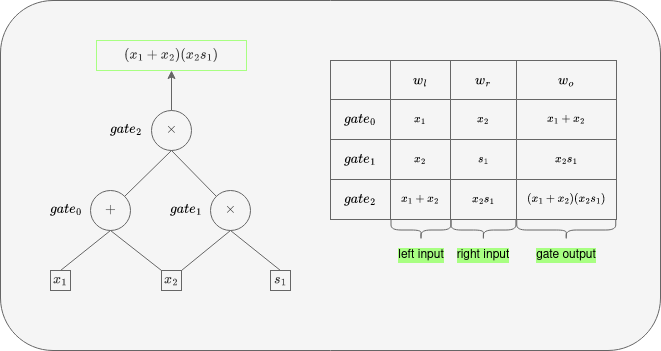
\includegraphics[width=1\linewidth]{figures/arithmetization.drawio.png}
    \caption{Toy Circuit}
    \label{fig:toy-circuit}
\end{figure}

The objective is to efficiently encode an arithmetic circuit into a set of polynomials. The first step is to encode each gate as an equation. Considering only gates for addition and multiplication, each gate could be written as one of the following:

\begin{align}
    \label{eq:primitive_gate_constraints}
    \text{\textit{addition:} } \text{left input} + \text{right input} = \text{gate output} 
    \\
    \text{\textit{multiplication:} } \text{left input} \times \text{right input} = \text{gate output}
\end{align}

That is a good start, but we could create an equation that can check the validity of both gate types. First, we denote the columns of the computational table as vectors $w_l, w_r, w_o$. By assigning $x_1 = 2, x_2 = 1, s_1 = 3$ for the \Cref{fig:toy-circuit} we get $w_l = [2, 1, 3], w_r = [1, 3, 3], w_o = [3, 3, 9]$. The values in the computation table represent the witness $(\publicinput, \witness)$, where $\publicinput$ are values of $x_1, x_2$ and the rest of the circuit is private $\witness$. 

To specify the type of the gate, we use selectors: $q_l$ left, $q_r$ right, $q_o$ output, $q_m$ multiplication, $q_c$ constant. These are vectors of size $n$ selecting the type of gate that we want to use. For example, if we are dealing with gate $i$, that is a multiplication gate, then $q_{m_i} = 1$; otherwise, it is always set to 0. The selectors could be combined to obtain the equation for gate $i$:

\begin{equation}
    \label{gate-constraint}
    w_{l_i}w_{r_i}q_{m_i} + w_{l_1}q_{l_i} + w_{r_i}q_{r_i} + w_{o_i}q_{o_i} + q_{c_i} + PI_i = 0
\end{equation}

Consider the example circuit and variable assignment $x_1 = 2, x_2 = 1, s_1 = 3$, and for simplicity, all unassigned selectors will have value 0. Then, it is possible to perform these operations:

\begin{itemize}
    \item \textit{addition:} $q_{l_i} = q_{r_i} = 1, q_{o_i} = -1$ \\
        For the addition gate, we want to keep only the addition and output terms of the equation. The rest will cancel out, thanks to the remaining selectors being 0.
    \item \textit{multiplication:} $q_{m_i} = 1, q_{o_i} = -1$ \\
        To engage a multiplication gate, we assign the selector such that only the multiplication and output terms of the equation remain.
    \item \textit{constant assignment:} \\
        Besides the operations of addition and multiplication, it is possible to do constant assignments (not illustrated on the example circuit). Say that we want the left input of a $gate_i$ to be equal to some constant $c$. To construct the equation for this gate, we can assign $q_{l_i} = 1, q_{c_i} = -c$, and the equation then simplifies to $w_{l_i} = c$, checking exactly what we want. This work, respectively, also for the right input, we just set the selectors as $q_{r_i} = 1, q_{c_i} = -c$.
\end{itemize}

$PI_i$ is public input, which is engaged only for the public input nodes (leaves of the graph). For all inner nodes, $PI_i = 0$. Notice that using the selector polynomial, some terms are canceled out so that we get to the separate gate constraints described in the beginning \eqref{eq:primitive_gate_constraints}. Below is a table with the explicit assignment of the selector for the specific example. 

% \begin{figure}[H]
%     \centering
%     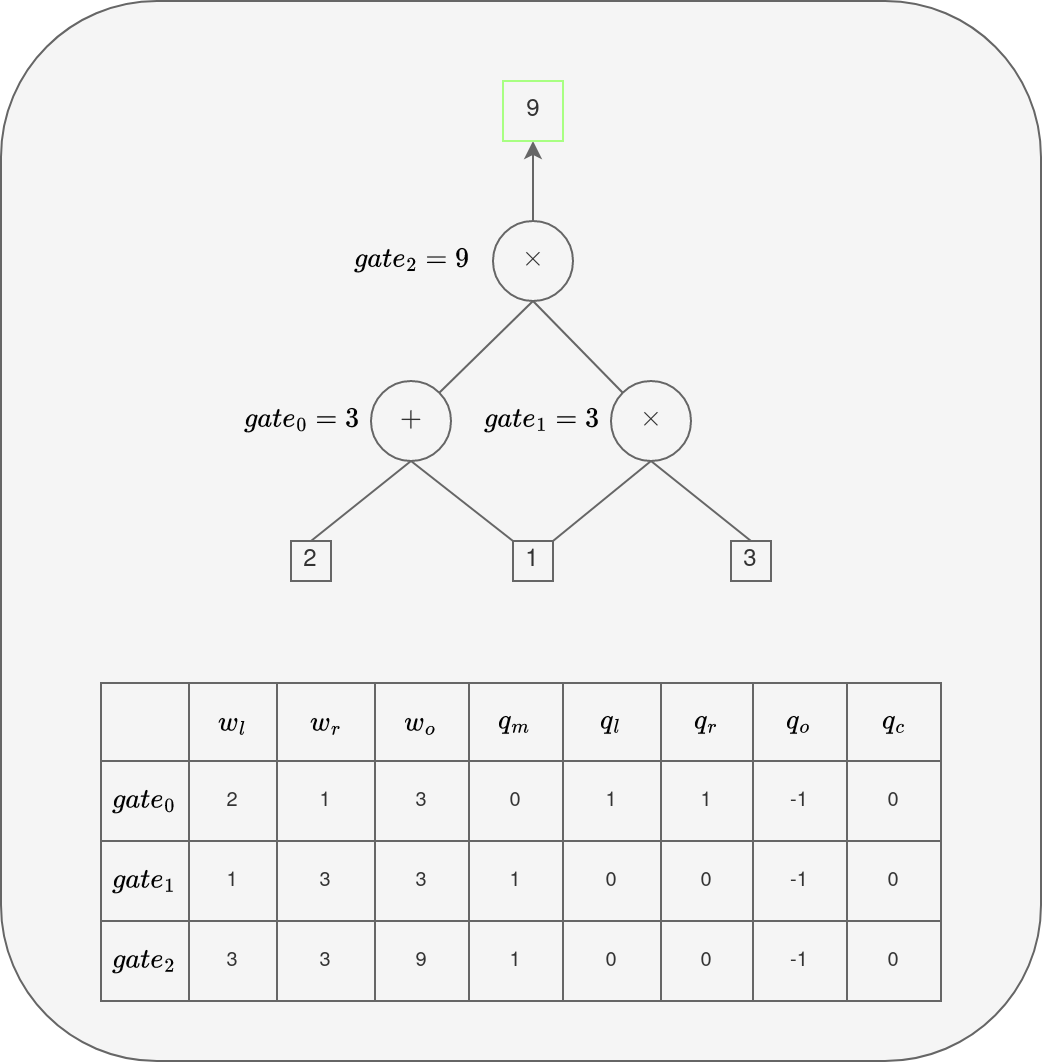
\includegraphics[width=0.75\linewidth]{figures/arithmetization_evaluated.drawio.png}
%     \caption{Evaluated diagram}
%     \label{fig:evaluated-circuit}
% \end{figure}

\begin{table}[H]
\begin{tabular}{|c|c|c|c|c|c|c|c|c|}
\hline
         & $w_l$ & $w_r$ & $w_o$ & $q_m$ & $q_l$ & $q_r$ & $q_o$ & $q_c$ \\ \hline
$gate_0$  & 2     & 1     & 3     & 0     & 1     & 1     & -1    & 0     \\ \hline
$gate_1$ & 1     & 3     & 3     & 1     & 0     & 0     & -1    & 0     \\ \hline
$gate_2$ & 3     & 3     & 9     & 1     & 0     & 0     & -1    & 0     \\ \hline
\end{tabular}
\end{table}

% Now we can get a bit closer to the arithmetization that is used in $\plonk$ we merge the witness vector $w_l, w_r, w_o$ into single $w$ such that: $$w_l = [w_0, \dots, w_{n-1}], w_r = [w_n, \dots, w_{2n-1}], w_o = [w_{2n}, \dots, w_{3n-1}]$$ 
% Now the witness $w$ encapsulates all of the values flowing through the circuit, where some of the values are public and some are secret. The verifier needs to check the output of the circuit and the public input, so naturally, these two will be public. The rest of the values remain private.

% To get the full gate equation we add one last thing. The public input to the circuit will be denoted by vector $PI$, remember that public input is a subset of the witness. In contrast to selector $q_c$, $PI$ can be changed for each execution of the circuit while 
% $q_c$ constants (surprisingly) remain bound to a specific circuit. For all (inner) nodes not related to input $PI$ will be set to 0. The full $\plonk$ gate equation looks like this:
% \begin{equation}\label{gate-constraint}
%     w_{i}w_{n+i}q_{m_i} + w_{i}q_{l_i} + w_{n+i}q_{r_i} + w_{2n+i}q_{o_i} + PI_i + q_{c_i} = 0 
% \end{equation}

% Let's revise this on our beloved Sudoku game. Imagine the prover is trying to convince the verifier that he knows the solution to a \href{https://en.wikipedia.org/wiki/Sudoku}{Sudoku problem}. Then the circuit is a program that checks if the Sudoku is filled validly and the prover wants to show that he can fill in such numbers that this program accepts his solution. Here the public input (public part of the witness) could be the initial state of the Sudoku problem as well as the dimensions of the board. Naturally private witnesses are the numbers that need to be filled in the board that the prover claims to know and does not want to share. We should also mention that there is a convention that the correct result of the circuit should be 0. That is the same as saying the output of the program is 0 if it succeeds.


\subsection{Transcription into polynomials}
It is possible to write express computation of each gate in the circuit as equation \Cref{gate-constraint}. But a much more elegant way is to condense all of the constraints into a single equation by interpolating the vectors.

\[
\begin{array}{cc}
    a(x) = \sum_{i=0} L_i(x)w_{l_i} & b(x) = \sum_{i=0} L_i(x)w_{r_i} \\
    c(x) = \sum_{i=0} L_i(x)w_{o_i} & q_l(x) = \sum_{i=0} L_i(x)q_{l_i}  \\
    q_{r_i}(c) = \sum_{i=0} L_i(x)q_{r_i} & q_m(x) = \sum_{i=0} L_i(x)q_{m_i}  \\
    q_{c_i}(x) = \sum_{i=0} L_i(x)q_{c_i} & PI(x) = \sum_{i=0} L_i(x)PI_i  \\
\end{array}
\]

This enables to represent gate constraints for the whole circuit $\CRKT$ as:
\begin{equation}
    \label{eq:gate-contraints}
    a(x)b(x)q_m(x) + a(x)q_l(x) + b(x)q_r(x) + c(x)q_o(x) + q_{c_i} + PI(x) = 0
\end{equation}

% This section was inspired by the lecture of Dan Boneh which is available on \href{https://zkhack.dev/whiteboard/}{ZK Whiteboard}. Since in the group of elliptic point we had only operation with addition and multiplication these will also be the only gates that we will use. Subtraction and division will be simulated by computing additive and multiplicative inverses. It is possible to work also with custom gates but for the simplicity this will be discussed in another section. For now we will consider only 2 binary gates. 

% Let's see how a specific circuit can be transformed into a polynomial. Take arithmetic operations $(x_1 + x_2)(x_2 + w_1)$ where $x$ are public inputs and $w$ is a secret witness. This can be visualized as a computation graph where the first sum is computed in addition $gate_0$, second sum in addition $gate_1$ and finally the product in $gate_2$.

% % \begin{table}[ht]
% %     \centering
% %     \begin{tabular}{ l | l l l}
% %      inputs:   & $x_1$ & $x_2$ & $w_1$       \\ 
% %      \hline
% %      $gate_0$: & $x_1$ & $x_2$ & $x_1 + x_2$ \\ 
% %      $gate_1$: & $x_2$ & $w_1$ & $x_2 + w_1$ \\ 
% %      $gate_2$: & $x_1 + x_2$ & $x_2 + w_1$ & $(x_1 + x_2)(x_2 + w_1)$ \\
% %     \end{tabular}
% %     \caption{Arithmetic circuit as a table}
% % \end{table}

% Notice how the first two columns show input and the third one output. The number in the right corner is 77 which is output of the arithmetic circuit. We set notation $|C|$ as number of gates in $C$, and also $|I| = |I_x| + |I_w|$ as number of public inputs plus number of private inputs. For case of binary gates the total number of elements in the computation trace is $d = 3|C| + |I|$ and we will also have set $\Omega = \{1, \omega, \omega^2, ..., \omega^{d-1} \}$. Now we are able to specify polynomial which partially represents the table. 

% In the original paper the each gate $i$ could be represented by a equation:

% $$q_{l_i} a_i + q_{r_i} b_i+ q_{o_i} c_i + q_{m_i} a_i b_i + q_{c_i} = 0$$

% where $a, b, c$ are left right and output wires and $q$ are selector polynomials. Specifically $q_l, q_r, q_o, q_m, q_c$ stand for left right output multiplication and constant, these are called selector and specify encode the structure of the circuit . Now for each gate we can perform three operations:
% \begin{itemize}
%     \item addition: by assigning 1 to selectors $q_l, q_r$, -1 to $q_o$ and 0 to remaining  
%     $a + b = c$
%     \item multiplication: by assigning 1 to $q_m$, -1 to $q_o$ and 0 to remaining $a \times b = c$
%     \item constant assignment: is done when binding to some public variable. we can bind it to the left variable by assigning $q_l = 1$, $q_c$ value we want to assign and rest is zero. $b = q_c$
% \end{itemize}

% \begin{table}[h]
%     \centering
%     \begin{tabular}{ l | l l l}
%      inputs:   & $t(\omega^{-1})= x_1$ & $t(\omega^{-2})=x_2$ & $t(\omega^{-3})=w_1$ \\ 
%      \hline
%      $gate_0$: & $t(\omega^{0})=x_1$  & $t(\omega^{1})=x_2$  & $t(\omega^{2})=x_1 + x_2$ \\ 
%      $gate_1$: & $t(\omega^{3})=x_2$  & $t(\omega^{4})=w_1$  & $t(\omega^{5})=x_2 + w_1$  \\ 
%      $gate_2$: & $t(\omega^{6})=x_1 + x_2$ & $t(\omega^{7})=x_2 + w_1$  & $t(\omega^{8})=(x_1 + w_2)(x_2 + w_1)$ 
%     \end{tabular}
%     \caption{Arithmetic circuit as a table}
% \end{table}

% % Now the polynomial will be interpolated. For example with FFT in time $d \log_2{d}$. This encoding has one flaw, can you spot it? We are not able to distinguish types of the polynomials and that is why we need selector polynomial. 

% To make this more succinct it would be nice to represent the whole circuit as a single polynomial. The key point to realize here is that system of equations in the same form could be interpreted as a single equation over polynomials. Suppose we have a vector like $v=(5,8,13)$. We can convert the vector into a list of points $(0,5),(1,8),(2,13)$ simply using the index of the value in the vector as the x-coordinate. Then there is a unique degree-2 polynomial function that passes through these points. Notice that we are entirely free to choose any domain we want. In $\plonk$ the polynomials are interpolated over the domain of roots of unity. The $n$-th root of unity is simply a group element that satisfies $x^n = 1$ and for $i<n, x^i \neq 1$. Let's have a set $\Omega = \{1, \omega, \omega^2, \omega^3 ..., \omega^n-1\}$

% To make this complete we need to realize that gate wire constraints $a, b, c$ are different for each of the equation and we can just transform them to polynomial to arrive to:
% $$L(x)a(x) + R(x)b(x) + O(x)\CRKT(x) + M(x)a(x)b(x) + O(x) + \CRKT(x) = 0$$


% By transcribing the problem we are reinterpreting the problem in terms of polynomial. We are asking the prover to give us witness $w$ such that together with the public input $x$ a specific program encoded circuit $C$ will give out some value. In the general case we are asking for such $w$ that $\CRKT(x,w) = 0$. Right now we will consider gates just with standard group operations. By that we mean addition and multiplication. In later sections we will see that it is also possible to construct $\plonk$ with custom gates, for now we will make our life easier by dealing only with binary gates.

% During the process of arithmetization the the $\verifier$ needs to make sure that $\prover$ did not cheat in any way. In particular we need to have gate constraints, which are equations between wires that are attached in the same gate. Secondly we will also want to have copy constraints that guarantee that for two consecutive gates the output of the first one is input to the second one. 


 
%%%  ===========================================================================
\section{Circuit checks}
\label{sec:checks}
We can encode arbitrary circuits with polynomials. The following objective is to convince the verifier that the prover knows such a secret witness $\witness$, for which $\CRKT(\publicinput, \witness) = 0$. The prover needs to guarantee the integrity of computing the circuit, and it turns out the verifier needs a lot of convincing since there are numerous ways to cheat. The prover needs to show that the following:
\begin{enumerate}
    \label{plonk-checks}
    \item correct public inputs are provided (input check)
    \item Gates are computed correctly (gate check)
    \item Gates are wired correctly (wiring check)
    \item The output of the circuit is zero (output check)
\end{enumerate}

Most of the checks are descriptive, besides the wiring check. Considering the example circuit \eqref{fig:toy-circuit}, this check ensures that outputs of $gate_0, gate_1$ are indeed provided as inputs to $gate_2$. This is also referred to as copy constraints because we want to make sure that the output of some gate is correctly copied to the input of another gate. Before proceeding to the implementation of this check, we will show how to perform zero tests on some domains.

\subsection{Zero Test}
\label{zero-test-on-h}

Observe that if some polynomial $f(x)$ is zero on $H$, then every element of $H$ has to be its root. A polynomial that has roots in all elements of the domain was denoted as $Z_H(x)$. That means we can factor the polynomial as $f(x) = g(x)Z_H(x)$. Therefore, if a polynomial is zero on $H$, it has to be divisible by the vanishing polynomial $Z_H(x)$. 

To put this into context, this test can be made into a standalone protocol with a polynomial commitment scheme. Below is a sketched diagram of how it works. In the $\plonk$ protocol, we will use this check, but the zero checks are not run independently on each polynomial. Instead, they are batched into the quotient polynomial $t(x)$ in \Cref{chap:round3}.

% % \pseudocodeblock{
% %   \textbf{Prover} \< \< \textbf{Oracle} \< \< \textbf{Verifier} \\
% %   \text{work} \< \< \< \< \\
% %   p(x), q(x) = p(x) / Z_H(x) \< \< \< \< \\
% %   \text{Add to transcript} \< \< \< \< \\
% %   \< \sendmessageright{top=transcript} \< \< \< \\
% %   \< \< z \gets \mathbb{F}_p \< \< \\
% %   \< \sendmessageleft{top=z} \< \< \< \\
% %   \< \sendmessagerightx{8}{p(z), q(z)} \< \\
% %   % \< \< \< \sendmessageright{top=Work result, bottom=Bottom message} \< \\
% %   \< \< \< \< \text{work} \\
% %   \< \< \< \< \text{verify KZG evaluation} \\
% %   \< \< \< \< Z_H(z) = z^n - 1 \\
% %   \< \< \< \< p(z) \stackrel{?}{=} q(z)Z_H(z) \\
% % }


% % %   \< \sendmessageright{top=transcript} \< \< \< \\
% % %   \< \< z \gets \mathbb{F}_p \< \< \\
% % %   \< \sendmessageleft{top=z} \< \< \< \\


% \begin{enumerate}
% \label{plonk-checks}
%     \item $P$ correctly encodes all of the inputs (input check)
%     \item Gates are computed correctly (gate check)
%     \item Gates are wired correctly (wiring check)
%     \item The output of the circuit is zero (output check)
% \end{enumerate}

% % % \hl{why is the input chosen such that the output is zero}

% Let $\omega \in \mathbb{F}_p$ be a primitive $k$-th root of unity for which $\omega^k = 1$. Then we can define a set $\Omega = \{1, \omega, \omega^2, ... \omega^{k-1}\}$ and $f \in \mathbb{F}_p^{\leq d} (X)$. Now there are some tasks, that prove might want to show to the verifier. Especially we will be interested into zero-test which shows that $f$ is identically zero on the set $\Omega$. This test uses a simple algebra fact:

% \begin{lemma}
%     $f$ is zero on $\Omega$ if and only if $f$ is divisible by $(x^k - 1)$
% \end{lemma}

% \begin{proof}
%     Let's start with reverse implication $\leftarrow$. If $f$ is divisible by $(x^k - 1)$ that means it can be factored into $f(x) = g(x)(x^k - 1)$. Now what happens if we plug some value of $\Omega$ into the function? For 1 it is obvious that the polynomial will result to zero and for others can be considered as $\omega^i, i<k$. Now using that fact that $\omega^k = 1$:
%     $$(x^k - 1) = ((\omega^{i})^k - 1) = ((\omega^{k})^i - 1) = (1^i - 1) = 0$$
    
%     $\rightarrow$ if $f$ is zero on $\Omega$ than plugging in any $\omega^i \in \Omega$ should result in zero and that is achieved when $f$ is divisible by $(x^k - 1)$ as seen in the previous case.
% \end{proof}

% This test can be transformed in a scheme. The prover would compute $q(x) = \frac{f(x)}{(x^k -1)}$ and will commit to $f, q$ using polynomial commitment scheme, which could be KZG. Then the verifier will sample a random $r \in \mathbb{F}_p$ and ask for evaluation of $f(r), q(r)$, the resulting verification will just compare: $f(r) = q(r)(r^k - 1)$. By % % \hl{lemma x} the probability that these polynomials are identical based on evaluation of a single point is sufficient. The verifier needs to compute $r^k$ which can be done in $O(log k)$

% Besides that a product check would be also very useful for us: $c = \prod_{\omega \in \Omega} f(\omega)$

% % % \hl{Perhaps add diagram for zero test}


\pseudocodeblock[head=Zero test]{
    \text{Prover } \prover \< \< \text{Verifer } \verifier \\
    \< \< \\[-0.5 \baselineskip]
    f(x), g(x) = f(x) / Z_H(x) \< \sendmessageright*{\relax[f]_1, [g]_1} \< \< \\
    \< \sendmessageleft*{z} \< z \gets \field \\
    \text{evaluate } f(z), g(z) \< \< \\
    \text{compute opening proofs } \pi_1, \pi_2 \< \< \\
    \< \sendmessageright*{f(z), g(z), \pi_1, \pi_2} \< \\
    \< \< \text{verify KZG openings } \pi_1, \pi_2 \\
    \< \< Z_H(z) = z^n - 1 \\
    \< \< f(z) \stackrel{?}{=} g(z)Z_H(z)
}

\begin{theorem}
    Zero-test is correct and computationally sound, assuming $\frac{d}{p}$ is negligible.
\end{theorem}

\label{is this sufficient?}
\begin{proof}
    We have already discussed the properties of KZG in \cref{chap:kzg} and the Schwartz-Zippel lemma in \Cref{comparing-poly}. 

    This check satisfies correctness because if $f(x)$ is zero on $H$, then it can be factored into $Z_H(x)g(x)$. The verifier can check the KZG opening and compare polynomials using the Schwartz-Zippel lemma.

    The zero test is also computationally sound because if the polynomial $f(x)$ is
    not zero on the whole domain $H$, then it cannot be divided by $Z_H(x)$. As a result, the prover cannot provide $g(x)$ that would satisfy $f(z) = g(z)Z_H(z)$ with non-negligible probability, which follows from the Schwartz-Zippel lemma.
\end{proof}


\subsection{Output Check}
Notice that the output of the circuit is always the output of the last gate of the circuit. This means the output of the circuit will be encoded as the last element of the witness. All the prover needs to do is show that $\CRKT(\omega^{n-1}) = 0$. This can be performed in a secure way using a polynomial commitment scheme where the verifier asks to open the polynomial $c(x)$ at $\omega^{n-1}$.

\begin{lemma}
    \label{output-correctness-soundness}
    The output check is correct and sound.
\end{lemma}

The properties of this check depend on the polynomial commitment scheme, and we have already discussed the validity of KZG in \Cref{chap:kzg}.

\subsection{Gate Check}
We have managed to encode the gate constraints by the equation  \Cref{eq:gate-contraints}. Using the zero test, it is possible to verify that $\forall x \in H:$
$$a(x)b(x)q_m(x) + a(x)q_l(x) + b(x)q_r(x) + c(x)q_o(x) + q_{c_i} + PI(x) = 0$$


\begin{lemma}
    \label{gate-correctness-soundness}
    The gate check is correct and computationally sound
\end{lemma}

\begin{proof}
    This follows from the properties of the zero test \Cref{zero-test-on-h}
\end{proof}

\subsection{Input Check}
We have encoded the public input is encoded using \Cref{eq:gate-contraints}. That means checking if correct public inputs were provided to the circuit can be encoded in the gate equation.

\begin{lemma}
    \label{input-correctness-soundness}
    The public input check is correct and sound
\end{lemma}

This follows from \Cref{gate-correctness-soundness}.

\subsection{Wiring Check}
\label{sec:wiring-check}
The structure of a circuit requires some values to be identical. The edges (wires) indicate that the output of the gate at one side should be passed as the input to the other gate. To ensure that the program is computed correctly, the prover needs to show that the values were copied correctly.

This check is performed using permutations. The structure of the circuit induces some equivalence classes. We will try to show that the copy constraints are satisfied by performing a permutation on the equivalence classes. For this purpose, we will choose rotation because it changes the position of every element. The diagram below \Cref{fig:permutation-function} shows how the permutation function would look for \Cref{fig:toy-circuit}.

\begin{figure}[H]
    \label{fig:permutation-function}
    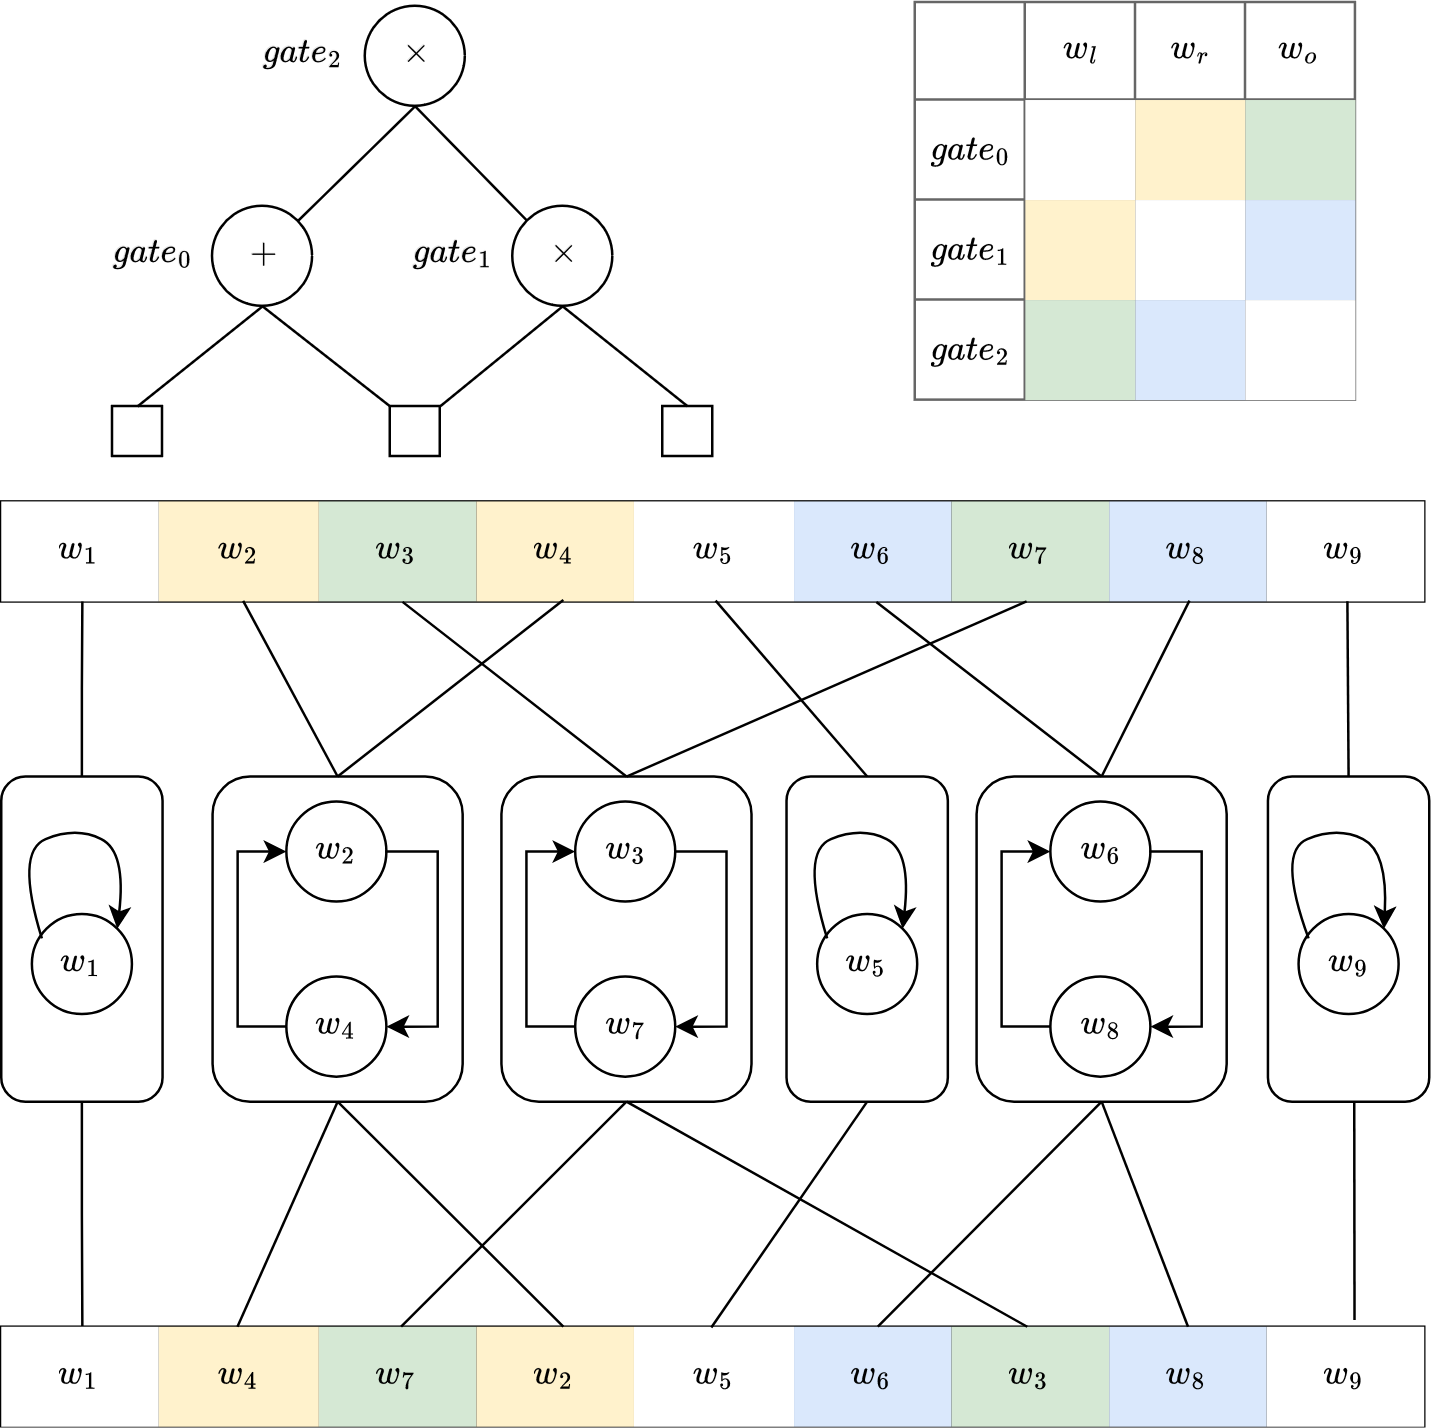
\includegraphics[width=0.75\linewidth]{round-figures/round2/permutation_function.drawio.png}
    \caption{Rotation of equivalence classes}
\end{figure}

It might look complicated, but essentially, we just did a clockwise rotation on the groups of variables of the circuit. Since we have changed the variables with equal values, the circuit should work the same as before and produce the same output. If all of the gate equations were true before the shuffling, then they would succeed also after this shuffling. On the other hand, if the prover did not do the arithmetization correctly and the gate wiring is not the same as in the former circuit, this check would detect it (with very high probability). That is the core idea that will be used in the permutation check.

\begin{lemma}
    \label{permutation-correctness-soundness}
    Consider vector $v = [v_1, v_2 \ldots v_n]$, constraints $v_i = v_j, v_k = v_l \ldots$ and a permutation function $\sigma$ that permutes the equivalence classes determined by the constraints. All of the contains are satisfied if and only if $v = \sigma(v)$.
\end{lemma}

\begin{proof}
    \textcolor{white}{there is nothing on this line:)}
    
    \begin{enumerate}
        \item[$\Rightarrow$] If all of the contains are satisfied and $\omega$ permutes only the indices inside the permutation classes, then the values remain unchanged. 
        \item[$\Leftarrow$]  If the vector remain unchanged after performing the permutation $\sigma$ then all of the elements in the equivalence classes induced by the permutation function must be the same and thus the constraints hold.
    \end{enumerate}
\end{proof}

